
\section{Smart SSD Architecture}\label{sec:ssdArch}

%In-storage computing (ISC, for short) is a new computing paradigm and has recently attracted notable attention. Unlike the traditional CPU-centric computing systems, it enables ISC devices to play a major role in computation by offloading key functions of host systems into ISC devices. This paradigm reflects well a recent computing trend toward~\textit{'insurrection of peripheral devices'}. This section describes our Smart SSD architecture and key components as ISC devices.

%SSD In-Storage Computing (ISC) is a new computing paradigm and has recently attracted notable attention. Unlike the traditional CPU-centric computing systems, it enables ISC devices to play a major role in computation by offloading key functions of host systems into ISC devices. This paradigm reflects a recent computing trend toward \emph{near-data processing}~\cite{Balasubramonian14}. This section describes our Smart SSD architecture and key components as ISC devices.

Smart SSDs, unlike the traditional CPU-centric computing systems, enable ISC devices to play a major role in computation by offloading key functions of host systems into ISC devices. Since its hardware architecture is identical to the aforementioned modern SSDs shown in Figure~\ref{fig:SSDInternals}, this section describes our Smart SSD software architecture and key components as ISC devices.



\begin{figure}[htbp]
%\vspace{-5mm}
	\centering
		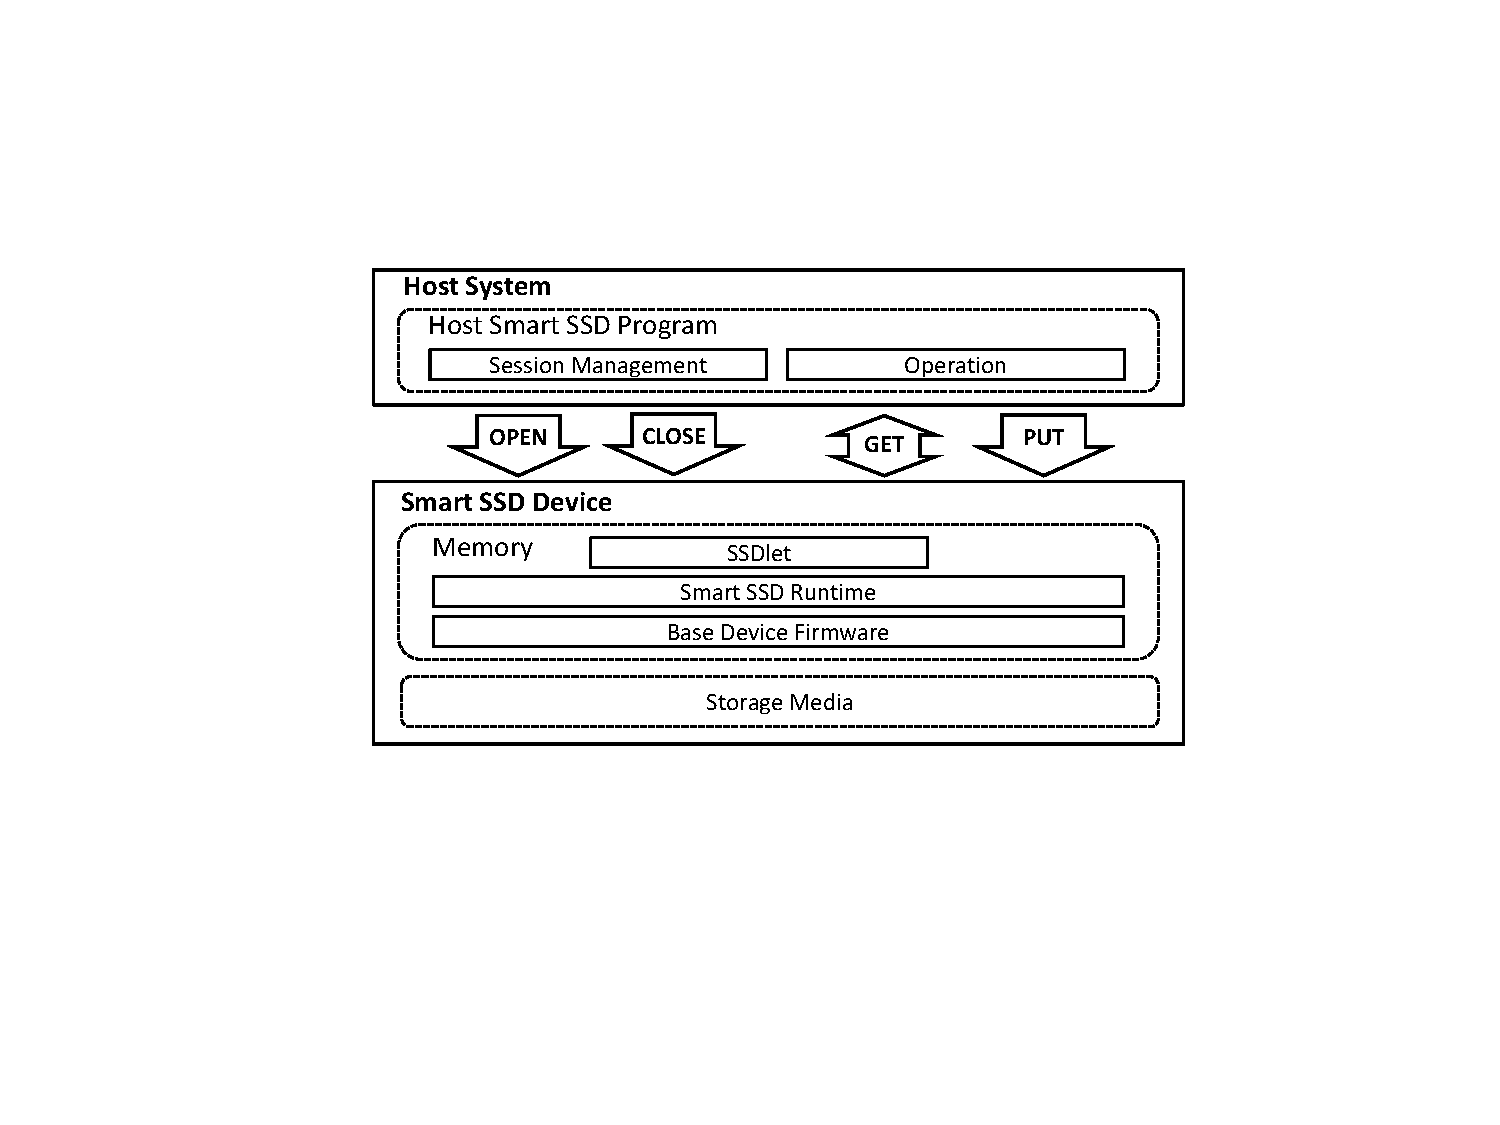
\includegraphics[width=0.9\columnwidth]{figures/SmartSSD_Architecture.pdf}
	\caption{\small Smart SSD Architecture}
	\label{fig:SmartSSD_arch}
\end{figure}

As illustrated in Figure~\ref{fig:SmartSSD_arch}, our Smart SSD consists of several key software components and it communicates with a Smart SSD host program via Smart SSD application programming models (APIs).


An SSDlet is a Smart SSD program in an ISC device. It implements application logic and responds to a Smart SSD host program. The SSDlet is executed in an event-driven manner by the Smart SSD runtime system. A Smart SSD runtime system connects the device Smart SSD program with a base device firmware, and implements the library of Smart SSD APIs. In addition, a base device firmware also implements normal I/O operations (read and write) of a storage device.

After an SSDlet is installed in the Smart SSD device, a host system runs the Smart SSD host program to interact with the SSDlet in the devices. This host program consists largely of two sections: a session management component and an operation component. The session component manages the lifetime of a session for Smart SSD applications so that the host Smart SSD program can launch an SSDlet by opening a session to the Smart SSD device. To support this session management, Smart SSD provides two APIs, namely, OPEN and CLOSE. Intuitively, OPEN starts a session and CLOSE terminates the existing session. Once OPEN starts a session, runtime resources such as memory and threads are assigned to run the SSDlet and a unique session ID is returned to the host Smart SSD program. Afterward, this session ID must be associated to interact the SSDlet. When CLOSE terminates the established session, it releases all the assigned resources and closes SSDlet associated with the session ID.

Once a session is established by OPEN, the operation component helps the host Smart SSD program interact with SSDlet in a Smart SSD device with GET and PUT APIs. This GET operation is used to check the status of SSDlet and receive output results from the SSDlet if the results are ready. This GET API implements the polling mechanism of the SAS/SATA interface because, unlike PCIe, such traditional block devices cannot initiate a request to a host such as interrupts. PUT is used to internally write data to the Smart SSD device without help from local file systems.


